%!TEX root =  cpt-rl-icml.tex

\pgfplotsset{every x tick label/.append style={font=\scriptsize}}

 \begin{figure*}
    \centering
		
		\hspace{-2em}
   \begin{minipage}{.26\textwidth}
\subfigure{
        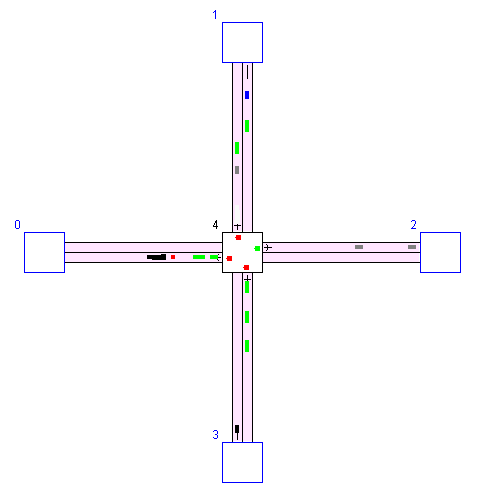
\includegraphics[width=1.9in,height=1.1in]{fig/road-net.png}
				}
				\caption{Snapshot of the road network from GLD simulator. The figure shows four edge nodes that generate traffic, one traffic light and  two-laned roads carrying automobiles.} 
\label{fig:road-net}

\end{minipage}
%%%%%%%%%%%%%%%%%%%%%%%%%%%%%%%%%%%%%%%
\begin{minipage}{.01\textwidth}
~ 
\end{minipage}
%%%%%%%%%%%%%%%%%%%%%%%%%%%%%%%%%%%%%%%
   \begin{minipage}{.64\textwidth}
     \begin{tabular}{cc}
\subfigure[AVG-SPSA]{
\label{fig:avg-hist}
\hspace{-2em} 
\tabl{c}{\scalebox{0.75}{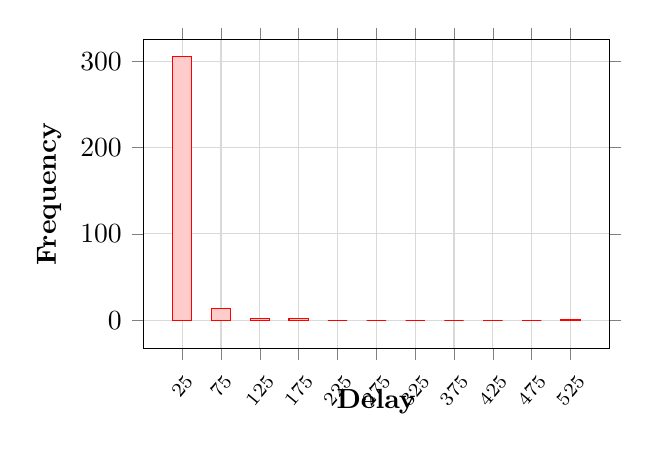
\begin{tikzpicture}
\begin{axis}[
ybar,
ymax=325,
%  legend style={at={(0.5,-0.2)},anchor=north,legend columns=-1},
legend pos=outer north east,
legend image code/.code={\path[fill=white,white] (-2mm,-2mm) rectangle
(-3mm,2mm); \path[fill=white,white] (-2mm,-2mm) rectangle (2mm,-3mm); \draw
(-2mm,-2mm) rectangle (2mm,2mm);},
ylabel={\bf Frequency},
xlabel={\textbf{Delay}},
x label style={at={(axis description cs:0.5,-0.1)},anchor=north},
symbolic x coords={0, 25,75,125,175,225,275,325,375,425,475,525, 12},
xmin={0},
xmax={12},
xtick=data,
ytick align=outside,
xticklabel style={rotate=50, align=center},
bar width=7pt,
%  bar shift=0pt,
%  enlarge x limits={abs=0.5},
% nodes near coords,
grid,
grid style={gray!30},
width=7.5cm,
height=5.5cm,
]
\addplot[red, fill=red!20]   coordinates { 
(25,306) (75,14) (125,2) (175,2) (225,0) (275,0) (325,0) (375,0) (425,0) (475,0) (525,1)   };
\end{axis}
\end{tikzpicture}}\\[0.5ex]}
}
&
%%%%%%%%%%%%%%%%%%%%%%%%%
\subfigure[CPT-SPSA]{
\label{fig:cpt-hist}
\hspace{-2em} 
\tabl{c}{\scalebox{0.75}{\begin{tikzpicture}
\begin{axis}[
ybar={2pt},
%  legend style={at={(0.5,-0.2)},anchor=north,legend columns=-1},
ymax=325,
legend pos=outer north east,
legend image code/.code={\path[fill=white,white] (-2mm,-2mm) rectangle
(-3mm,2mm); \path[fill=white,white] (-2mm,-2mm) rectangle (2mm,-3mm); \draw
(-2mm,-2mm) rectangle (2mm,2mm);},
ylabel={\bf Frequency},
xlabel={\textbf{Delay}},
x label style={at={(axis description cs:0.5,-0.1)},anchor=north},
symbolic x coords={0, 5,15,25,35,45,55,65,75,85,95,105,115,125,135,145,155,165,175, 17},
xmin={0},
xmax={17},
xtick=data,
ytick align=outside,
xticklabel style={rotate=50, align=center},
bar width=7pt,
% nodes near coords,
grid,
grid style={gray!30},
width=7.5cm,
height=5.5cm,
]
\addplot[darkgreen, fill=darkgreen!20]   coordinates {  
(5,113) (15,94) (25,49) (35,27) (45,18) (55,3) (65,3) (75,1) (85,2) (95,0) (105,1) (115,0) (125,1) (135,1) (145,0) (155,0)
}; 
 

\end{axis}
\end{tikzpicture}}\\[0.5ex]}
}
\end{tabular}
\caption{Histogram of the sample delays for the path from node $0$ to $1$ (see Figure \ref{fig:road-net}) for AVG-SPSA that minimizes overall expected  delay and CPT-SPSA that maximizes CPT-value of differential delay. }
\label{fig:histogram-perf}
\end{minipage}
\end{figure*}

%%%%%%%%%%%%%%% End Hist %%%%%%%%%%%%%%%%%

We consider a traffic signal control application where the aim is to improve the road user experience by an adaptive traffic light control (TLC) algorithm.
We apply the CPT-functional to the delay experienced by road users, since CPT realistically captures the attitude of the road users towards delays. We then optimize the CPT-value of the delay and contrast this approach with traditional expected delay minimizing algorithms. It is assumed that the CPT functional's parameters $(u,w)$ are given (usually, these are obtained by observing human behavior). The experiments are performed using the GLD traffic simulator \cite{GLDSim}, and the implementation is available at \url{https://bitbucket.org/prashla/rl-gld}.

% \subsection{Simulation Setup}  
We consider a road network with $\N$ signalled lanes that are spread across junctions and $\M$ paths, where each path connects (uniquely) two edge nodes, from which the traffic is generated (see Figure \ref{fig:road-net}). 
%\todoc{Can we have a higher quality figure?}
At any instant $n$, let $q_n^i$ and $t_n^i$ denote the queue length and elapsed time since the lane turned red, for any lane $i = 1,\ldots, \N$. Let $d_n^{i,j}$ denote the delay experienced by $j$th road user on $i$th path, for any $i=1,\ldots,\M$ and $j=1,\ldots,n_i$, where $n_i$ denotes the number of road users on path $i$.
We specify the various components of the traffic control MDP below.
The state $s_n=(q_n^1,\ldots,q_n^{\N},t_n^1,\ldots,t_n^{\N},d_n^{1,1},\ldots,d_n^{\M,n_{\M}})\tr$ is a vector of lane-wise queue lengths, elapsed times and pathwise delays. Any combination of traffic lights that can simultaneously be switched to green constitutes an action in the MDP.
% The actions are the feasible traffic signal configurations. 

 %\begin{figure}
    %\centering
        %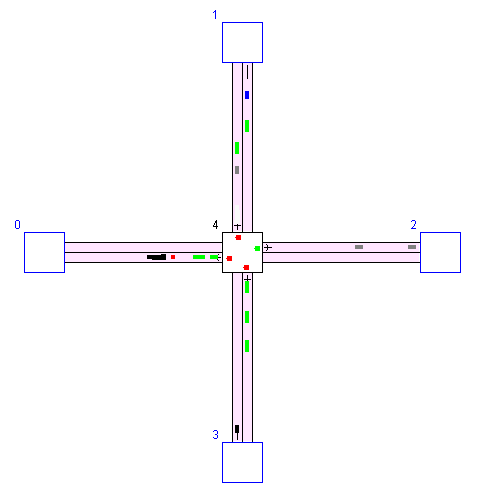
\includegraphics[width=2in,height=1.1in]{fig/road-net.png}
%\caption{Snapshot of the road network from GLD simulator. The figure shows four edge nodes that generate traffic, one traffic light and  two-laned roads carrying automobiles.}
%\label{fig:road-net}
%\end{figure}



\pgfplotsset{every x tick label/.append style={font=\scriptsize}}

 \begin{figure*}
    \centering
     \begin{tabular}{cc}
\subfigure[Expected delay (path-wise) for AVG-SPSA and CPT-SPSA]{
\label{fig:avg}
\hspace{-2em} 
\tabl{c}{\scalebox{0.6}{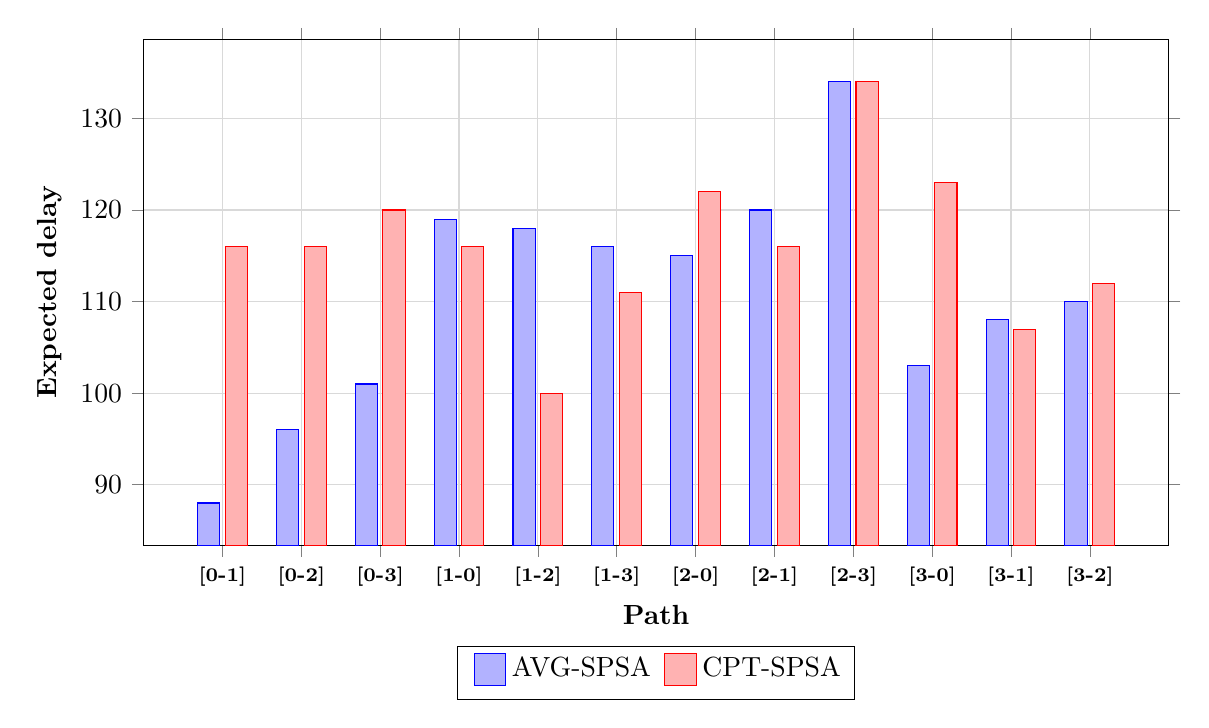
\begin{tikzpicture}
\begin{axis}[
ybar={2pt},
  legend style={at={(0.5,-0.2)},anchor=north,legend columns=-1},
%legend pos=outer north east,
legend image code/.code={\path[fill=white,white] (-2mm,-2mm) rectangle
(-3mm,2mm); \path[fill=white,white] (-2mm,-2mm) rectangle (2mm,-3mm); \draw
(-2mm,-2mm) rectangle (2mm,2mm);},
ylabel={\bf Expected delay},
xlabel={\textbf{Path}},
symbolic x coords={0, 1, 2, 3, 4, 5, 6, 7, 8, 9, 10, 11, 12, 13},
xmin={0},
xmax={13},
xtick=data,
ytick align=outside,
xticklabels={{\bf [0-1],\bf [0-2],\bf [0-3],\bf [1-0],\bf [1-2],\bf [1-3],\bf [2-0],\bf [2-1],\bf [2-3],\bf [3-0],\bf [3-1],\bf [3-2],}},
xticklabel style={align=center},
bar width=8pt,
%nodes near coords,
grid,
grid style={gray!30},
width=14.6cm,
height=8cm,
]
\addplot   coordinates {  (1,88) (2,96) (3,101) (4,119) (5,118) (6,116) (7,115) (8,120) (9,134) (10,103) (11,108) (12,110)}; 
\addlegendentry{AVG-SPSA}
\addplot coordinates {  (1,116) (2,116) (3,120) (4,116) (5,100) (6,111) (7,122) (8,116) (9,134) (10,123) (11,107) (12,112)}; 
\addlegendentry{CPT-SPSA}
\end{axis}
\end{tikzpicture}}\\[1ex]}
}
&
%%%%%%%%%%%%%%%%%%%%%%%%%
\subfigure[CPT of differential delay (pathwise) for AVG-SPSA and CPT-SPSA]{
\label{fig:cpt}
\hspace{-2em} 
\tabl{c}{\scalebox{0.6}{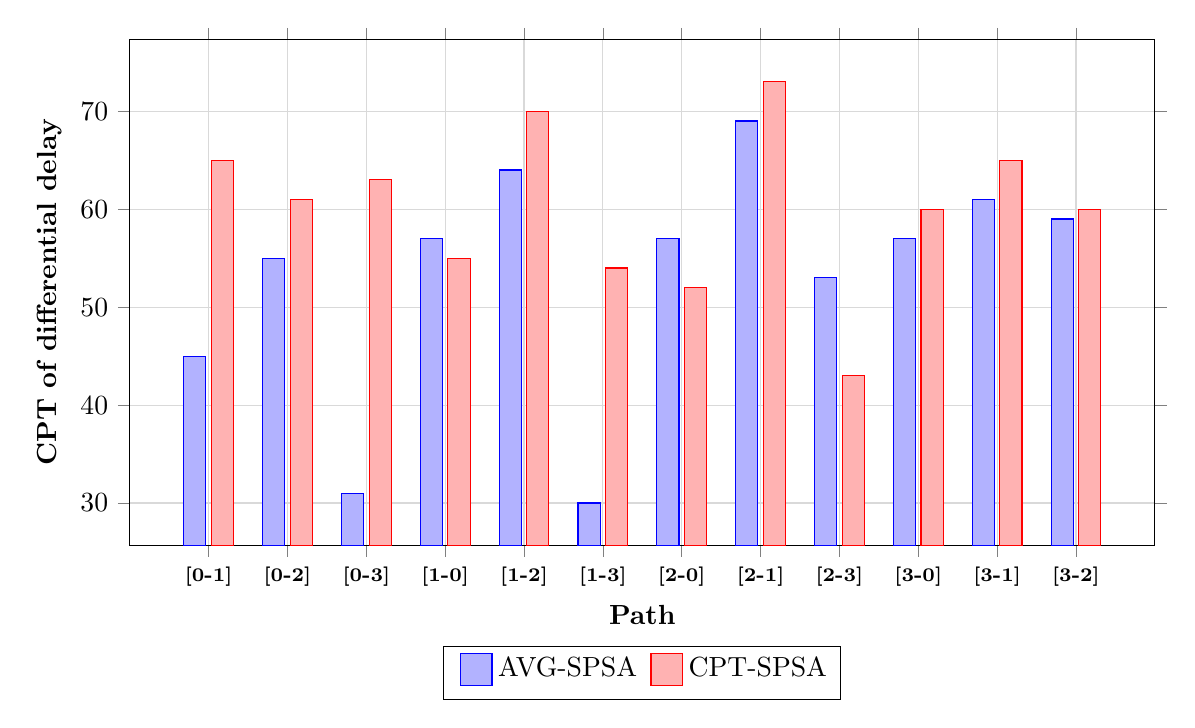
\begin{tikzpicture}
\begin{axis}[
ybar={2pt},
  legend style={at={(0.5,-0.2)},anchor=north,legend columns=-1},
%legend pos=outer north east,
legend image code/.code={\path[fill=white,white] (-2mm,-2mm) rectangle
(-3mm,2mm); \path[fill=white,white] (-2mm,-2mm) rectangle (2mm,-3mm); \draw
(-2mm,-2mm) rectangle (2mm,2mm);},
ylabel={\bf CPT of differential delay},
xlabel={\textbf{Path}},
symbolic x coords={0, 1, 2, 3, 4, 5, 6, 7, 8, 9, 10, 11, 12, 13},
xmin={0},
xmax={13},
xtick=data,
ytick align=outside,
xticklabels={{\bf [0-1],\bf [0-2],\bf [0-3],\bf [1-0],\bf [1-2],\bf [1-3],\bf [2-0],\bf [2-1],\bf [2-3],\bf [3-0],\bf [3-1],\bf [3-2],}},
xticklabel style={align=center},
bar width=8pt,
%nodes near coords,
grid,
grid style={gray!30},
width=14.6cm,
height=8cm,
]
\addplot   coordinates {  (1,45) (2,55) (3,31) (4,57) (5,64) (6,30) (7,57) (8,69) (9,53) (10,57) (11,61) (12,59) 
}; 
\addlegendentry{AVG-SPSA}
\addplot coordinates {  (1,65) (2,61) (3,63) (4,55) (5,70) (6,54) (7,52) (8,73) (9,43) (10,60) (11,65) (12,60) 
}; 
\addlegendentry{CPT-SPSA}
\end{axis}
\end{tikzpicture}}\\[1ex]}
}
\end{tabular}
\caption{AVG and CPT values for two algorithms on each of the $12$ paths in Figure \ref{fig:road-net}: AVG-SPSA minimizes overall expected  delay (see \eqref{eq:avg-traffic}), while CPT-SPSA maximizes CPT-value of differential delay (see \eqref{eq:cpt-traffic}). }
\label{fig:avg-cpt-perf}
\end{figure*}

We consider Boltzmann policies that have the form
$$
\pi_{\theta}(s,a) = \frac{e^{\theta^{\top} \phi_{s,a}}}{\sum_{a' \in {\A(s)}} e^{\theta^{\top} \phi_{s,a'}}},
\hspace{6pt} \forall s \in \S,\;\forall a \in \A(s),
$$
with features $\phi_{s,a}$ as described in Section V-B of \cite{prashanth2012threshold}.
% We consider two different notions of return as follows:
% %
% \textbf{CPT:} 
For any policy $\theta$, let $X_i^\theta$ be the delay r.v. and $\mu_i^\theta$ the proportion of road users along path $i$, for $i=1,\ldots,\M$. 
Any road user along path $i$ will evaluate the delay (s)he experiences in a manner that is captured well by CPT. 
An important component of CPT is to employ a reference point to calculate gains and losses. 
%Choosing a suitable reference point is challenging, but \cite{tversky1992advances} advocate using status-quo as the reference point. 
In our setting, we use pathwise delays, say $B_i$ for path $i$, obtained from a pre-timed TLC (cf. the Fixed TLCs in \cite{prashanth2011reinforcement}) as the reference point.
If the delay of any TLC algorithm is less than that of pre-timed TLC, then the (positive) difference in delays is perceived as a gain and in the complementary case, the delay difference is perceived as a loss. Thus, the CPT-value $\C(B_i-X_i)$ for any path $i$ in \eqref{eq:cpt-traffic} is to be understood as a \textit{differential delay} w.r.t. $B_i$.  
Now, the objective is to maximize the weighted sum of CPT-values across paths, i.e., 
% With the objective of maximizing the experience of road users across paths, the overall return to be optimized is given by
\begin{align}
\max_{\theta \in \Theta} \text{CPT}(X_1^\theta,\ldots,X_{\M}^\theta) = \sum_{i=1}^{\M} \mu_i^\theta \C(B_i - X_i^\theta),\label{eq:cpt-traffic}
\end{align}
where $\Theta$ is the $d$-dimensional hypercube formed by intervals $[0.1,1.0]$ in each dimension. The rationale behind the objective above is that CPT-value $\C(B_i - X_i^\theta)$ would capture the road user experience/satisfaction for each path $i$ and the goal is to maximize the \textit{average satisfaction} over all paths.  
% where  $\C(B_i-X_i)$ is the CPT-value along path $i$ for differential delay r.v. $B_i-X_i$. 
% \textbf{EUT:} Here we only use the utility functions $u^+$ and $u^-$ to handle gains and losses, but do not distort probabilities. 
% Thus, the EUT objective is defined as
% \begin{align*}
% \text{EUT}(X_1,\ldots,X_{\M}) = \sum_{i=1}^{\M} \mu^i \left(\E(u^+(X_i) - \E(u^-(X_i)\right),
% \end{align*}
% where $\E(u^+(X_i)) = \intinfinity \Prob{u^+(X_i)>z} dz$ and $\E(u^-(X_i)) - \intinfinity \Prob{u^-(X_i)>z} dz$, for $i=1,\ldots,\M$.

For the sake of comparison, we consider the traditional objective of minimizing the overall average delay, i.e.,
\begin{align}
\min_{\theta\in \Theta}\text{AVG}(X_1^\theta,\ldots,X_{\M}^\theta) = \sum_{i=1}^{\M} \mu_i^\theta \E(X_i^\theta). \label{eq:avg-traffic} 
\end{align}
In comparison to CPT objective, the above does not incorporate baseline delays, makes no distinction between gains and losses via utility functions and does not distort probabilities. 
%Thus, the AVG objective is defined as
%\begin{align}
%\text{AVG}(X_1,\ldots,X_{\M}) = \sum_{i=1}^{\M} \mu^i \E(X_i).
%\end{align}   
%where $\E(X_i) = \intinfinity P(u^+(X_i)>z) dz - \intinfinity P(u^-(X_i)>z) dz$.
% An important component of CPT is to employ a reference point to calculate gains and losses. 
% %Choosing a suitable reference point is challenging, but \cite{tversky1992advances} advocate using status-quo as the reference point. 
% In our setting, we use path-wise delays obtained from a pre-timed TLC (cf. the Fixed TLCs in \cite{prashanth2011reinforcement}) as the reference point. If the delay of any TLC algorithm is less than that of pre-timed TLC, then the (positive) difference in delays is perceived as a gain and in the complementary case, the delay difference is perceived as a loss. Thus, the CPT-value $\C(X_i)$ for any path $i$ in \eqref{eq:cpt-traffic} is to be understood as a \textit{differential delay}.  
% 
% %, as the road network considered is high-dimensional (state space cardinality $> 10^{60}$). 
% 
% Using a Boltzmann policy that has the form
% $$
% \pi_{\theta}(s,a) = \frac{e^{\theta^{\top} \phi_{s,a}}}{\sum_{a' \in {\A(s)}} e^{\theta^{\top} \phi_{s,a'}}},
% \hspace{6pt} \forall s \in \S,\;\forall a \in \A(s),
% $$
% with features $\phi_{s,a}$ as described in Section V-B of \cite{prashanth2012threshold},
% 

We implement the following TLC algorithms:

{\bf\em CPT-SPSA}: This is a first-order algorithm (see Algorithm \ref{alg:1spsa}) that solves \eqref{eq:cpt-traffic} using SPSA-based gradient estimates and the scheme from Algorithm \ref{alg:holder-est} for estimating CPT-value \\$\C(B_i-X_i)$ for each path $i=1,\ldots,\M$, with $d_n^{i,j}, j=1,\ldots,n_i$ as the samples.

% {\bf\em EUT-SPSA}: This is similar to CPT-SPSA, except that weight functions $w^+(p)=w^-(p)=p,$ for $p\in [0,1]$. 

{\bf\em AVG-SPSA}: This is SPSA-based first-order algorithm that solves \eqref{eq:avg-traffic}, while using sample averages of the delays to estimate the expected delay $\E(X_i)$ for each path $i=1,\ldots,\M$. 

The underlying CPT-value $\C(X_i), \forall i$ follows the exact form as in section \ref{sec:expts-simple}, except here we set $\lambda = 2.25$.
The choices for $\lambda$, $\sigma$, $\eta_1$ and $\eta_2$ are based on median estimates given by \cite{tversky1992advances} and have been used earlier in a traffic application (see \cite{gao2010adaptive}).
For all the algorithms,
 motivated by standard guidelines (see \cite{spall2005introduction}),
 we set $\delta_n = 1.9/n^{0.101}$ and $a_n = 1/(n+50)$. The initial point $\theta_0$ is the $d$-dimensional vector of ones and $\forall i$, the operator $\Gamma_i$ keeps the iterate $\theta_i$ bounded within $[0.1, 1.0]$.

\begin{table}
 \centering
  \caption{AVG and CPT-value estimates for AVG-SPSA and CPT-SPSA algorithms. Note: CPT-value is of differential delays w.r.t. pre-timed TLC, while 
  AVG-value uses absolute delays.}
  \label{tab:cpt-results}
 \begin{tabular}{|c|c|c|}
  \toprule 
   & \textbf{AVG-value}& \textbf{CPT-value }\\\midrule
   AVG-SPSA & $\bm{111.67}$ & $-17.63$ \\\midrule
   CPT-SPSA & $116.21$ & $\bm{21.12}$\\
   \bottomrule
  \end{tabular}
%   
%   \vspace{1ex}
%   
\end{table}


 
The experiments involve two phases:
first, a training phase where we run each algorithm for $500$ iterations, with each iteration involving two perturbed simulations. Each simulation involves running the traffic simulator with a fixed policy parameter for $5000$ steps and this corresponds to approximately $4000$ delay samples. The training phase is followed by a test phase where we fix the policy obtained at the end of training and then run the traffic simulator with the aforementioned parameter for $5000$ steps. The results presented are averages over ten independent simulations.

% \subsection{Results} 

Table \ref{tab:cpt-results} presents the overall AVG and CPT-values for AVG-SPSA and CPT-SPSA, while Figures \ref{fig:avg}--\ref{fig:cpt} present the expected delay and CPT of differential delay for each of the $12$ paths in Figure \ref{fig:road-net}.  
We observe that AVG-SPSA exhibits a better AVG-value, while CPT-SPSA shows a higher CPT value. 
Further, from Figure \ref{fig:histogram-perf} that presents the histograms of the delays for the path from $0$ to $1$, we observe that CPT-SPSA results in a strategy that avoids high delays at the cost of a slightly higher average delay, whereas AVG-SPSA has a few sample delays are significantly larger than the average delay. 
%the average  While the results in Table \ref{tab:cpt-results} are aggregated over all the paths in Figure \ref{fig:road-net}, we also analyze the delays over each path for both algorithms. 
% A similar exercise for pre-timed TLC resulted in a CPT-value of $-46.14$. 
%It is evident that each algorithm converges to a different policy and the difference, in $\ell_1$ norm, between policy parameters obtained at the end of training phase for AVG-SPSA and CPT-SPSA was observed to be $6.51$. 
% As shown in Table \ref{tab:cpt-results},  AVG-SPSA results in a TLC policy with lower expected delay, while CPT-SPSA's policy has higher CPT-value. This is expected because AVG-SPSA uses neither utilities nor probability distortions and minimizes overall delay, while CPT-SPSA uses a pre-timed TLC baseline and treats delay gains and losses differently. 
%We observe that CPT-SPSA gives significantly better CPT-value, while on the remaining $7$ paths, the CPT-value of CPT-SPSA and AVG-SPSA are comparable. From an expected delay viewpoint, AVG-SPSA exhibits lower expected delay on $4$ paths, while on the remaining paths the expected delay of AVG-SPSA and CPT-SPSA	are comparable. 


% esp. in the light of previous findings which show CPT matches human evaluation well and there is a need for algorithms that serve human needs well.
%\todoc{It would be nice to point out how the CPT policy is different than the others.}

